\section{Funktionsorientierte Testverfahren}

\begin{tcolorbox}
    \textbf{Funktionsorientierte Tests} werden in allen Testphasen des \textbf{V-Modells}\footnote{s. Abschnitt~\ref{sec:v-modell}} durchgeführt mit dem Ziel, die in den Spezifikationen festgehaltene  Funktionalität vollständig gegenzuprüfen.\\
    Sie testen das Verhalten eines \textbf{Testgegenstands}, also einer \textit{Methode}, einer \textit{Klasse} oder eines (Sub-)Systems.
\end{tcolorbox}
\vspace{2mm}

\noindent
Im Folgenden werden Verfahren beschrieben, mit denen funktionsorientierte Tests effektiv gestaltet werden können.

\subsection{Funktionale Äquivalenzklassen}\label{subsec:funktionale-aquivalenzklassen}
Die Vielfältigkeit möglicher Eingabefolgen in Software übersteigt oft die Umsetzbarkeit in Testfälle.\\
\textbf{Äquivalenzklassen} beruhen auf der Idee, dass viele Eingabemöglichkeiten von dem System auf die gleiche Art und Weise bearbeitet werden.

\begin{tcolorbox}[title=Äquivalenzklassen]
    \blockquote[{\cite[43]{Wed09c}}]{
    Die unterschiedlichen Bereiche, in denen ein Testgegenstand gleichartig reagiert, werden Äquivalenzklassen genannt.
    }\\
    \textbf{Gültige Äquivalenzklassen} stellen hierbei zulässige Elemente dar, die vom Testgegenstand verarbeitet werden sollen, \textbf{ungültige Äquivalenzklassen} hingegen Elemente, die vom Testgegenstand abgelehnt werden sollen.
\end{tcolorbox}

\noindent
Sinnvollerweise werden Äquivalenzklassen zur Identifikation durchnummeriert.

\subsubsection*{Beispiel}
Ein Programm berechnet den zu gewährenden Rabatt bei einem Einkauf:
\begin{itemize}
    \item $2\%$ Rabatt werden bei einem Einkauf ab € $1000,-$ gewährt
    \item Beträge $<= 0$ lösen eine Fehlermeldung aus
    \item für einen Betrag $x$ mit $0 < x < 1000$ werden unterschiedliche Rabatte berechnet
\end{itemize}

Hieraus können folgende Äquivalenzklassen ermittelt werden:

\begin{itemize}
    \item \textbf{Gültige Äquivalenzklassen}
    \begin{itemize}
        \item[] \textbf{(1a)} Betrag $0 < x < 1000 $
        \item[] \textbf{(1b)} Betrag $\geq 1000 $
    \end{itemize}
    \item \textbf{Ungültige Äquivalenzklassen}
    \begin{itemize}
      \item[] \textbf{(1c)} Betrag $\leq 0 $
    \end{itemize}
\end{itemize}

\subsubsection*{Typen von Äquivalenzklassen}
\textit{Wedemann} empfiehlt die Einteilung von Äquivalenzklassen in Kategorien (vgl.~\cite[43]{Wed09c}):

\begin{enumerate}
    \item \textbf{Wertebereich}, z.B. Zeiträume
    \item \textbf{Aufzählungen}, z.B. Familienstand
    \item \textbf{Voraussetzungen}, z.B.bei Passworteingaben: Eine Ziffer, einen Großbuchstaben
\end{enumerate}

\subsubsection*{Tests mit Stellvertretern einer Äquivalenzklasse}
Die Tests verwenden dann aus jeder Äquivalenzklasse einen \textbf{Stellvertreter}.
Es wird unterschieden nach

\begin{itemize}
    \item \textbf{Gutfälle}: Tests, in denen nur Stellvertreter aus gültigen Äquivalenzklassen verwendet werden
    \item \textbf{Schlechtfälle}: Tests, in denen nur Stellvertreter aus ungültigen Äquivalenzklassen verwendet werden
\end{itemize}

\noindent
Mit o.a. Beispiel lassen sich somit 3 konkrete Stellvertreter definieren:

\begin{itemize}
    \item \textbf{Gutfälle}:
    \begin{itemize}
        \item (1a) € $12,-$
        \item (1b) € $2000,-$
    \end{itemize}
    \item \textbf{Schlechtfälle}:
    \begin{itemize}
        \item (1a) € $-26,-$
    \end{itemize}
\end{itemize}

\subsection*{Mehrere Äquivalenzklassen pro Eingabe}
Oft können mögliche Eingabewerte nach unterschiedlichen Kriterien in verschiedene Äquivalenzklassen gruppiert werden.\\
Als Beispiel führt \textit{Wedemann} die Eingabe eines Passworts an: Das Passwort muss
\begin{itemize}
    \item aus mindestens 8 Zeichen bestehen
    \item[] und
    \item mindestens einen Buchstaben enthalten
    \item[] und
    \item mindestens eine Zahl enthalten
\end{itemize}

\noindent
Es ergeben sich folgende Äquivalenzklassen:

\begin{itemize}
    \item \textbf{Anzahl der Zeichen}:
    \begin{itemize}
        \item[] \textbf{gültig} (1a) 8 oder mehr Zeichen
        \item[] \textbf{ungültig} (1b) weniger als 8 Zeichen
    \end{itemize}
    \item \textbf{Mindestens ein Buchstabe und eine Zahl}:
    \begin{itemize}
        \item[] \textbf{gültig} (2a) ein Buchstabe und eine Zahl
        \item[] \textbf{ungültig}
        \begin{itemize}
            \item[] (2b) keine Zahl
            \item[] (2c) keine Buchstaben
        \end{itemize}
    \end{itemize}
\end{itemize}

\subsubsection*{Testdaten}
Um zu verhindern, dass ein Fehler durch einen anderen maskiert wird, muss nun \textit{jede} Äquivalenzklasse mindestens einmal im Test so vorkommen, dass alle anderen Äquivalenzklassen gültig sind (vgl.~\cite[44]{Wed09c}).
Mit o.a. Beispiel ergibt sich das folgende Stellvertreter:

\begin{itemize}
    \item \textbf{Gutfälle}
    \begin{itemize}
        \item[] (1a) (2a) \textit{abcd1234§}
    \end{itemize}
    \item \textbf{Schlechtfälle}
    \begin{itemize}
        \item[] (1b) (2a) \textit{ab12§}
        \item[] (1a) (2b) \textit{abcdefgh§}
        \item[] (1a) (2c) \textit{1234567§}
    \end{itemize}
\end{itemize}

\vspace{2mm}
\begin{tcolorbox}[colback=white]
    Es werden ausschliesslich Gutfälle/Gutfälle und Gutfälle/Schlechtfälle kombiniert.
    Schlechtfälle/Schlechtfälle werden nicht kombiniert, da man davon ausgeht, das dabei nur in Sonderfällen neue Fehler entdeckt werden, aber dadurch die Anzahl der Testfälle zu stark ansteigt.
\end{tcolorbox}
\vspace{2mm}

\subsubsection*{Mehrere Eingaben}
Gibt es \textbf{mehrere Eigaben} wird genauso vorgegangen wie bei zwei Gruppen von Äquivalenzklassen pro Eingabe: Jede Äquivalenzklasse muss mindestens einmal im Test vorkommen, wobei alle anderen Äquivalenzklasse gültig sind (vgl.~\cite[44]{Wed09c}).\\
Als Beispiel führt \textit{Wedemann} die Eingabe von \textit{Vorname} und \textit{Nachname} an (vgl.~\cite[44]{Wed09c}): Ein Vorname und ein Nachname muss aus mindestens 2 Zeichen bestehen, woraus sich folgende Äquivalenzklassen ergeben:

\begin{itemize}
    \item \textbf{Vorname}
    \begin{itemize}
        \item \textbf{Gültige Äquivalenzklassen}
        \begin{itemize}
            \item[] \textbf{(1a)} 2 oder mehr Zeichen
        \end{itemize}
        \item \textbf{Ungültige Äquivalenzklassen}
        \begin{itemize}
            \item[] \textbf{(1b)} weniger als 2 Zeichen
        \end{itemize}
    \end{itemize}
    \item \textbf{Nachname}
    \begin{itemize}
        \item \textbf{Gültige Äquivalenzklassen}
        \begin{itemize}
            \item[] \textbf{(2a)} 2 oder mehr Zeichen
        \end{itemize}
        \item \textbf{Ungültige Äquivalenzklassen}
        \begin{itemize}
            \item[] \textbf{(2b)} weniger als 2 Zeichen
        \end{itemize}
    \end{itemize}
\end{itemize}

\noindent
Die Testdaten sind dann:

\begin{itemize}
    \item \textbf{Gutfälle}
    \begin{itemize}
        \item[] (1a) (2a) ``\textit{Max}`` ``\textit{Moritz}``
    \end{itemize}
    \item \textbf{Schlechtfälle}
    \begin{itemize}
        \item[] (1a) (2b) ``\textit{Max}`` ``\textit{M}``
        \item[] (1b) (2a) ``\textit{M}`` ``\textit{Moritz}``
    \end{itemize}
\end{itemize}

\begin{tcolorbox}[colback=white]
    Auch hier gilt: Kombinationen von ungültigen Äquivalenzklassen werden nicht getestet, weshalb (1b) (2b) nicht in den Testdaten auftaucht.
\end{tcolorbox}

\subsubsection*{Mehrere Eingaben und mehrere Gruppen von Äquivalenzklassen}
Bei realen Anforderungen mit \textbf{mehreren Eingaben und mehreren Gruppen von Äquivalenzklassen} pro Eingabe wird genauso wie bei den o.a. Beispielen vorgegangen.
Dadurch ist auch bei einer größeren Anzahl von Äquivalenzklassengruppen eine noch überschaubare Anzahl der konstruierten Testfälle gewährleistet (vgl.~\cite[45]{Wed09c}).

\subsubsection*{Grenzwertanalyse}
Es ist sinnvoll, an den \textbf{Grenzen von Äquivalenzklassen} zu testen, da hier erfahrungsgemäß Fehler auftreten.\\
Mit o.a. Beispiel der Rabattberechnung würden sich unter Berücksichtigung der Grenzwerte  folgende Testfälle ergeben:

\begin{itemize}
    \item \textbf{Gutfälle}:
    \begin{itemize}
        \item (1a) € $1$, € $999,-$
        \item (1b) € $1000,-$
    \end{itemize}
    \item \textbf{Schlechtfälle}:
    \begin{itemize}
        \item (1a) € $0,-$
    \end{itemize}
\end{itemize}

\noindent
Für die gültige Äquivalenzklasse (1a) ist ein Gutfall hinzugekommen.\\
Tatsächlich bedeutet die Berücksichtigung von Grenzwerten von Äquivalenzklassen, dass meistens mehr Testfälle hinzukommen.\\
Es bietet sich dann nach Möglichkeit an, die Testfälle so zu gestalten, dass die verschiedenen Grenzwerte in unterschiedlichen Testfällen gleichzeitig geprüft werden.\\
In dem Beispiel mit den mehreren Eingaben (Vorname, Nachname)könnten die Testdaten folgendermaßen aussehen:

\begin{itemize}
    \item \textbf{Gutfälle}
    \begin{itemize}
        \item[] (1a) (2a) ``\textit{hu}`` ``\textit{li}``
    \end{itemize}
    \item \textbf{Schlechtfälle}
    \begin{itemize}
        \item[] (1a) (2b) ``\textit{hu}`` ``\textit{l}``
        \item[] (1b) (2a) ``\textit{h}`` ``\textit{li}``
    \end{itemize}
\end{itemize}

\subsubsection*{Test spezieller Werte}
\texbf{Spezielle Eingebewerte} verursachen häufig Probleme, weshalb diese mit dem \textbf{Test spezieller Werte} geprüft werden:

\begin{itemize}
    \item wird mit Zahlen gerechnet, wird häufig die $0$ als Testdatum verwendet, um Probleme bei der Division aufzudecken
    \item bei der Verarbeitung von Zeichenketten kann der leere String \code{""} Probleme verursachen
    \item bei Datenbankanwendungen werden SQL-Schlüsselwörter in den Testdaten verwendet
    \item Schalttage bzw. die Umstellung von Sommer-/Winterzeit wird bei Datumsberechnungen als spezielle Werte verwendet
\end{itemize}

\subsubsection*{Grenzen des Verfahrens}
Auch wenn die Methode der Äquivalenzklassen eine etablierte, ausgereifte Methode darstellt, ist ihr Einsatz schwierig, wenn das Verhalten vom Zustand abhängt - in diesen Fällen verwendet man \textbf{zustandsbasierte Tests} (s. Abschnitt~\ref{subsec:zustandsbasierter-test}).

\subsubsection*{Ursache-Wirkungs-Analyse}
Besitzen Äquivalenzklassen untereinander Abhängigkeiten, weil sich bspw. Eingaben gegenseitig bedingen, wird es schwer, Testdaten vernünftig zu konstruieren.\\
\textit{Wedemann} gibt hierzu exemplarisch das Beispiel eines Tests für einen Geldautomaten an, der nur Geld auszahlen soll, wenn die Karte gültig, die PIN richtig und genügend Geld auf dem Konto vorhanden ist; ist die PIN korrekt und die Karte gültig, soll ein anderer Betrag eingegeben werden können; die Karte soll eingezogen werden, wenn die PIN falsch ist und es sich um den dritten Versuch der Eingabe der PIN handelt. Für diesen Fall sei das Verfahren der \textbf{Ursache-Wirkungs-Analyse} geeignet (vgl.~\cite[46]{Wed09c}); \textit{Wedemann} verweist in diesem Zusammenhang auf \cite{ST05}.


\subsection{Zustandsbasierter Test}\label{subsec:zustandsbasierter-test}
Wenn eine Methode einer Klasse bei unterschiedlichen Feldern ein anderes Verhalten zeigt, ist das Verhalten von dem \textbf{inneren Zustand abhängig}.\\
Da sich dies auf Testgegenstände auswirkt, muss das unterschiedliche Verhalten in den verschiedenen Zuständen getestet werden.\\
\textit{Wedemann} führt als Beispiel in \cite[46 ff.]{Wed09c} einen Stack an, bei dem die Methoden \code{push()} / \code{pop()} / \code{top()} anderes Verhalten zeigen, je nachdem, ob der Stack gefüllt (\textit{filled}), leer (\textit{empty}) oder voll (\textit{full}) ist:

\begin{minted}{java}
class Stack {
    public Stack(int maxSize){...}
    public boolean isEmpty(){...}
    public int size(){...}
    public Object top() throws EmptyStack{...}
    public void push(Object o) throws FullStack{...}
    public void pop() throws EmptyStack{...}
    ...
}
\end{minted}

\subsubsection*{Zustände und Zustandsübergänge}
Für einen \textbf{vollständigen Test} muss nicht nur das Verhalten in allen Zuständen z.B. anhand von allen \textbf{Äquivalenzklassen} getestet werden, sondern auch alle \textbf{Zustandsänderungen}: Hierbei werden nicht bloß die \textit{definierten} Zustandsänderungen getestet, sondern es wird auch versucht, für den Testgegenstand nicht erlaubte Zustandsänderungen zu provozieren, um die Möglichkeit diesbzgl. auszuschließen und somit evtl. späteren Fehler vorzubeugen. \\

\begin{tcolorbox}[colback=white]
    Eine oft übersehene Fehlerquelle ist das sog. \textbf{temporal coupling}: Eine Methode ist von dem Zustand des Objektes abhängig und funktioniert korrekt, wenn das Objekt vorher durch eine andere Operation in einen entsprechenden Zustand versetzt wurde; liegt der Zustand nicht vor, erfolgt u.U. keine korrekte Berechnung (vgl.\cite[44 f.]{Mar08} sowie \cite[259]{Mar08}):

    \begin{minted}{java}
private Object calculate() {
    this.computationBase = calculateBase();
    this.result = calculateValue();

    return result;
}

private Object calculateValue() {
    ComputatioBase base = this.computationBase;

    if (base.leastSigificantBit() == 0) {
        ...
    }
    ...
}
    \end{minted}

    \noindent
    Das \textbf{hidden temporal coupling} sorgt in diesem Fall dafür, dass wahrscheinlich ein falsches Ergebnis berechnet wird, wenn zuerst \code{calculateValue()} aufgerufen wird, ohne, das vorher \code{calculateBase()} ausgeführt wurde.\\

     \noindent
     Eine mögliche Lösung für dieses Problem könnte durch ein Refactoring erfolgen:
    \begin{minted}{java}
// calculateBase wird in jedem Fall ausgeführt, wenn
// die Berechnung des Ergebnisses angefordert wird
private Object calculateBaseAndValue() {
    this.computationBase = calculateBase();

    if (this.computationBase.leastSigificantBit() == 0) {
        this.result = ...
    } else {
        this.result = ...
    }

    return this.result;
}
    \end{minted}
\end{tcolorbox}


\noindent
In einfachen Fällen können die benötigten Testfälle ohne Formalismus erraten werden; für kompliziertere Fälle wird ein systematisches Vorgehen benötigt, damit nichts übersehen wird.\\
Hierzu wird zunächst ein \textbf{UML-Zustandsdiagramm} (s. Abschnitt~\ref{ch:zustandsautomaten}) der Zustände und ihrer Zustandsübergänge erstellt (s. Abbildung~\ref{fig:popstate}), woraufhin dann eine Zustandsübergangstabelle (s. Tabelle~\ref{tab:popstate}) erstellt wird, aus der alle Zustände und Ereignisse mit ihren Folgezuständen abgelesen werden können.

\vspace{5mm}
\begin{tcolorbox}[colback=red!20,title={Notation für \textit{Event[Guard]}}]
    \textit{Wedemann} verwendet den Doppelpunkt ``:`` als Separator für die Notation \textit{Event[Guard]} (lies: ``das Ereignis wird getriggert, wenn der Guard zu $true$ evaluiert.``) in Abbildung~\ref{fig:popstate}.\\
    Für diese Notation findet sich in \cite[320 f.]{OMG17} kein Hinweis.
\end{tcolorbox}
\vspace{5mm}

\begin{figure}
    \centering
    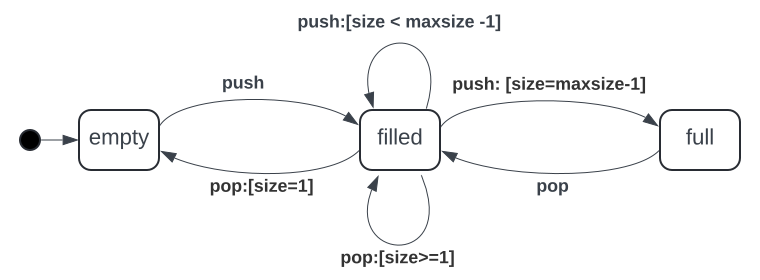
\includegraphics[scale=0.5]{part four/Testende Verfahren/img/popstate}
    \caption{UML-Zustandsdiagramm für Objekte der Klasse \textit{Stack}. (Quelle: in Anlehnung an \cite[Abb. 5.1, 47]{Wed09c})}
    \label{fig:popstate}
\end{figure}

\begin{table}[]
    \centering
    \setlength{\tabcolsep}{0.5em}
    \def\arraystretch{1.5}
    \begin{tabular}{|l|c|l|c|}
        \hline
        & \textbf{empty}                                                                     & \multicolumn{1}{c|}{\textbf{filled}}                                                                          & \textbf{full}                                                                     \\ \hline
        \code{push()} & filled                                                                             & \begin{tabular}[c]{@{}l@{}}{[}size\textless{}maxsize-1{]}: filled\\ {[}size = maxsize-1{]}: full\end{tabular} & \begin{tabular}[c]{@{}c@{}}full\\ \textless{}Exception\textgreater{}\end{tabular} \\ \hline
        \code{pop()}  & \begin{tabular}[c]{@{}c@{}}empty\\ \textless{}Exception\textgreater{}\end{tabular} & \begin{tabular}[c]{@{}l@{}}{[}size>1{]} : filled\\ {[}size=1{]}: empty\end{tabular}                       & filled                                                                            \\ \hline
    \end{tabular}
    \caption{Zustandsübergangstabelle für das Beispiel \textit{Stack}. Die Inhalte der Tabelle sind die Folgezustände; in spitzen Klammern stehen die Ergebnisse bei verbotenen Übergängen. (Quelle: \cite[Tab. 5.1, 48]{Wed09c})}
    \label{tab:popstate}
\end{table}

\noindent
Für den Test müssen in allen Zuständen die Methode \code{isEmpty()}, \code{size()} und \codde{top()} getestet werden, die den Zustand nicht verändern, woraus sich bereits $9$ Tests ergeben.\\
Anhand der Zustandsübergangstabelle müssen alle Zustandsübergänge getestet werden, woraus sich $8$ weitere Tests ergeben.\\
Die Aufgabe der Tester hierbei ist es, einen oder mehrere Pfade zufinden, die dies mit möglichst geringem Aufwand ermöglichen (vgl.~\cite[48]{Wed09c}): Für das o.a. Beispiel wäre das ein Stack mit \code{maxsize=3}, bei dem $4$-mal \code{push()} und $3$-mal \code{pop()} hintereinander aufgerufen wird.

\subsubsection*{Zustände}
\textit{Wedemann} merkt an, das sich bei dieser Diskussion die Frage ergeben kann, ``was denn nun genau unter einem Zustand zu verstehen ist`` (\cite[48]{Wed09c}): Ist ein Zustand bereits durch jedes Attribut, das über \code{set()} verändert werden kann, gegeben? \textit{Wedemann} bejaht dies: ``[...] auch ein Attributwert [ist] als Zustand zu sehen und der Test ist vollständig, wenn ein gesetzter Wert auch verwendet wird.`` (\cite[48]{Wed09c}).
Er fügt allerdings an, dass es für solch einfache Fälle nicht notwendig sei, den vorgestellten Formalismus zu verwenden, da dieser nur sinnvoll bei Klassen sei, bei denen ``es mehrere Zustände gibt, in denen sich die Methoden so unterschiedlich verhalten, dass dies mit Äquivalenzklassen nicht mehr abgebildet werden kann`` (\textit{ebenda}).